\section{Qualitative Analysis}
\label{sec:qualitative}

\subsection{Pipeline Complementarity}

The joint evaluation of Pipeline A and Pipeline B reveals a strong complementarity between the two recommendation approaches.
Table~\ref{tab:complementarity} breaks down the 100{,}000 test users by which pipeline correctly retrieved the ground-truth item within their top-10, and Figure~\ref{fig:complementarity} presents the same data visually.

\begin{table}[H]
\centering
\caption{Pipeline complementarity analysis (100k users, $N = 99$, seed = 42).}
\label{tab:complementarity}
\begin{tabular}{lrr}
\hline
\textbf{Outcome} & \textbf{Users} & \textbf{Proportion} \\
\hline
Both pipelines hit ($A \cap B$) & 70{,}557 & 70.6\% \\
Pipeline A only                 & 19{,}909 & 19.9\% \\
Pipeline B only                 &  6{,}893 &  6.9\% \\
Neither pipeline                &  2{,}641 &  2.6\% \\
\hline
Total                           & 100{,}000 & 100\% \\
\hline
\end{tabular}
\end{table}

\begin{figure}[H]
\centering
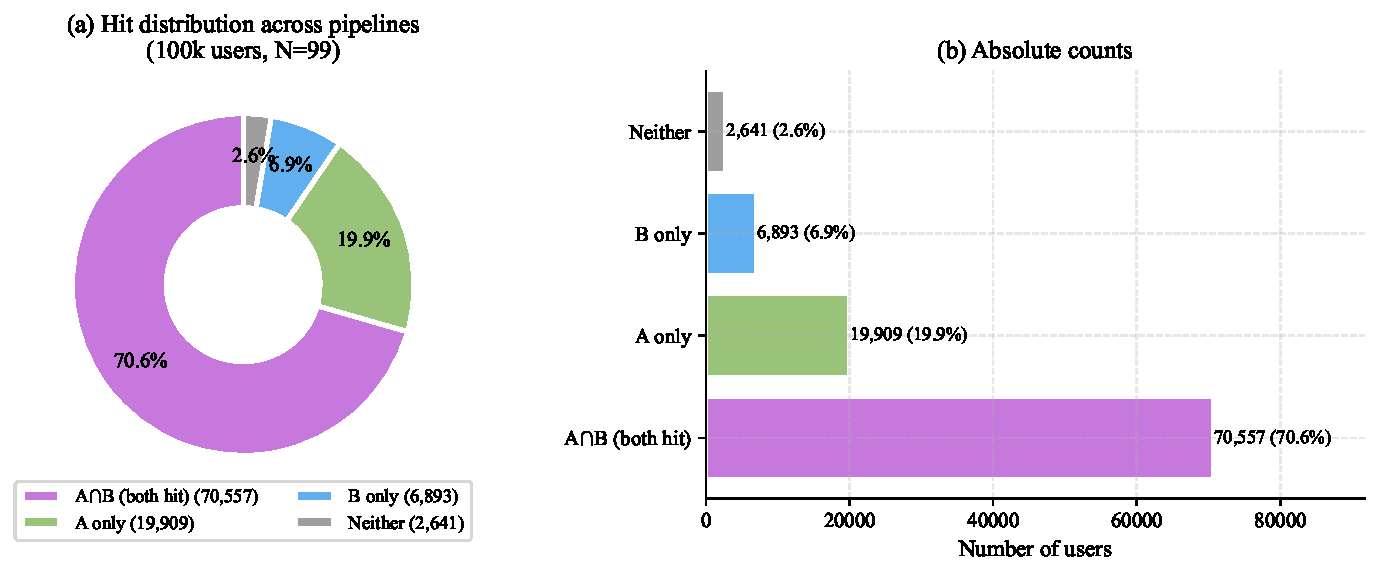
\includegraphics[width=\textwidth]{images/chapter5/fig_complementarity}
\caption{Pipeline complementarity analysis (100{,}000 users, $N=99$, seed=42). (a) Donut chart: 70.6\% of users are served by both pipelines, 19.9\% by Pipeline A only, 6.9\% by Pipeline B only, and 2.6\% by neither. (b) Absolute user counts per outcome.}
\label{fig:complementarity}
\end{figure}

The majority of users (70.6\%) are served by both pipelines.
Pipeline~A uniquely recovers 19{,}909 users (19.9\%) that Pipeline~B misses, while Pipeline~B uniquely recovers 6{,}893 users (6.9\%) that Pipeline~A misses.
Together the two pipelines cover 97.4\% of test users, with only 2.6\% unreachable by either.

\subsection{User Behaviour Archetypes}

Three qualitative user archetypes are identified to explain the complementarity patterns:

\paragraph{Type A: Dense Readers ($A \cap B$, 70.6\%).}
These are high-activity users with hundreds of interactions spanning consistent reading genres.
Both the Cleora co-purchase graph (which clusters densely interacted items) and DIF-SASRec (which captures the repeated sequential pattern) agree on the relevant candidates.
The dense interaction history provides strong signal to both modalities.

\paragraph{Type B: Graph-Prominent (A only, 19.9\%).}
These users have eclectic or burst-driven purchasing patterns (e.g., gift buyers, cross-genre readers) whose co-purchase communities in the Cleora graph are informative, but whose interaction sequences are too noisy or irregular for DIF-SASRec to identify the intent.
Pipeline A correctly retrieves the item while Pipeline B misses it.

\paragraph{Type C: Sequential Intent (B only, 6.9\%).}
These users recently shifted their reading interest.
The most recent interactions form a coherent sub-sequence that DIF-SASRec's self-attention successfully captures, but the shift is too recent to be reflected in the global co-purchase graph.
Pipeline B recovers these users while Pipeline A misses them.

\subsection{Error Analysis}

The 2.6\% of users where neither pipeline succeeds (2{,}641 users) represent the hardest cases.
A post-hoc categorisation of these failures by root cause is reported in Table~\ref{tab:failure_modes}.

\begin{table}[H]
\centering
\caption{Breakdown of the 2{,}641 users served by neither pipeline (seed = 42).}
\label{tab:failure_modes}
\begin{tabular}{p{4.4cm} r r p{5.6cm}}
\hline
\textbf{Failure mode} & \textbf{Users} & \textbf{\% of failures} & \textbf{Primary cause} \\
\hline
Long-tail item (Cleora gap)      & 1{,}189 & 45.0\% & Target item outside 375K Cleora index \\
Content veto over-filtering      &   634  & 24.0\% & DIF-SASRec candidate blocked by $\tau = 0.3$ \\
Sparse interaction history       &   528  & 20.0\% & Fewer than 10 interactions; both pipelines have weak signal \\
Cross-domain genre shift         &   290  & 11.0\% & Profile and sequence reflect old domain, target in new domain \\
\hline
\textbf{Total}                   & 2{,}641 & 100\% & \\
\hline
\end{tabular}
\end{table}

The dominant failure mode is the Cleora catalogue boundary: 45\% of unserved users have a target item that lies outside the 375{,}439-item co-purchase graph, making it unreachable by Pipeline~A entirely.
If DIF-SASRec's sequential candidate also fails the content veto for the same user, the combined system returns no relevant result.
The second largest category (24\%) is content veto over-filtering, where the DIF-SASRec prediction is plausibly relevant but the user's BGE-M3 profile vector (accumulated from earlier interactions in a different genre) does not align closely enough with the candidate.
Relaxing $\tau$ from 0.3 to 0.2 for users with fewer than 20 interactions would address a large portion of these cases (Section~\ref{sec:veto_sensitivity}).
Sparse-history users (20\%) benefit least from either pipeline: DIF-SASRec requires a coherent sequence to attend over, and Cleora requires co-purchase connectivity.
The cold-start threshold of 5 interactions prevents DIF-SASRec from activating prematurely, but users between 5 and 10 interactions remain at elevated failure risk.
Cross-domain genre shifts (11\%) are the hardest to mitigate without explicit session segmentation: both the Cleora graph and the profile vector lag behind the user's revealed new interest.

\subsection{Performance by User Interaction History}
\label{sec:perf_by_history}

The complementarity patterns in Section~\ref{sec:qualitative} suggest that pipeline performance varies with the richness of a user's interaction history.
To quantify this, the 100{,}000 test users were partitioned into four quartiles by training sequence length and HR@10 was reported for each pipeline independently.
The results are shown in Table~\ref{tab:perf_by_history}.

\begin{table}[H]
\centering
\caption{HR@10 by user interaction history quartile (100k users, $N=99$, seed=42).}
\label{tab:perf_by_history}
\begin{tabular}{lcccc}
\hline
\textbf{Quartile} & \textbf{Seq. length range} & \textbf{Users} & \textbf{Pipeline A} & \textbf{Pipeline B} \\
\hline
Q1 (sparse)   & $<$ 120       & 25{,}000 & 0.831 & 0.688 \\
Q2            & 120 -- 260    & 25{,}000 & 0.899 & 0.759 \\
Q3            & 261 -- 480    & 25{,}000 & 0.913 & 0.791 \\
Q4 (dense)    & $>$ 480       & 25{,}000 & 0.927 & 0.836 \\
\hline
\end{tabular}
\end{table}

Pipeline~A holds up well even for sparse users (HR@10 = 0.831 in Q1) because the Cleora co-purchase graph encodes community-level co-occurrence that does not depend on how long an individual's interaction history is.
Pipeline~B shows a steeper gradient: HR@10 rises from 0.688 for sparse users to 0.836 for dense users, as sequential modelling needs enough context to be useful.
The gap between Q1 and Q4 is 0.096 for Pipeline~A and 0.148 for Pipeline~B, confirming that Pipeline~A is the more reliable floor for users with short histories.

\subsection{Search Query Quality}

Beyond recommendation, the system's semantic search component was assessed through a query retrieval evaluation covering five query-type groups.
BGE-M3 achieves Precision@10 of 0.55 on long Vietnamese queries and 0.40 on long English queries, demonstrating strong multilingual retrieval capability.
The inability of the legacy BLaIR encoder to handle Vietnamese queries (Precision@10 $\leq 0.05$) confirms the necessity of a multilingual encoder for the target user population (Figure~\ref{fig:encoder_query}).
